\documentclass[12pt]{report}  

\pagestyle{empty}

\usepackage{graphics}
\usepackage{amsmath,amssymb,amsthm, multicol,array}
\usepackage[pdftex]{graphicx}
\usepackage{enumerate}
\usepackage{epsf}

\theoremstyle{definition}
\newtheorem{thm}{Theorem}
\newtheorem{lem}[thm]{Lemma}
\newtheorem{cor}[thm]{Corollary}
\newtheorem{rem}[thm]{Remark}
\newtheorem{remark}[thm]{Remark}
\newtheorem{conj}[thm]{Conjecture}
\newtheorem{definition}[thm]{Definition}

\newcommand{\naturals}{\mathbb{N}}
\newcommand{\integers}{\mathbb{Z}}
\newcommand{\complex}{\mathbb{C}}
\newcommand{\reals}{\mathbb{R}}
\newcommand{\mcal}[1]{\mathcal{#1}}
\newcommand{\rationals}{\mathbb{Q}}
\newcommand{\Aut}{\text{Aut}}
\newcommand{\Lp}[2]{\left\|{#1}\right\|_{L^{#2}}}
\newcommand{\tr}{\text{tr}}
\newcommand{\field}{\mathbb{F}}

\addtolength{\oddsidemargin}{-.75in}
\addtolength{\evensidemargin}{-.75in}
\addtolength{\textwidth}{1.5in}
\addtolength{\topmargin}{-1in}
\addtolength{\textheight}{2.25in}

\begin{document}
\begin{center}
{\bf \Large Math 13 - Week 4: Induction and the Pigeonhole Principle}
\vspace{0.2cm}
\hrule
\end{center}

\begin{enumerate}	

\item Let $n\in \naturals$. Prove that there exist positive integers $a$ and $b$, with $a\neq b$, such that $n^a - n^b$ is divisible by 10. For example, if $n = 17$, then
\[
	17^6 - 17^2 = 24137569-289 = 24137280.
\]
\textit{Hint: Consider the numbers $n^1, n^2, \ldots, n^{11}$ and look at the ones digits.}

\vfill

\item Prove that the sum of the first $n$ odd natural numbers is $n^2$.
\vfill

\item What is wrong with the following proof?

\begin{thm}
	$\frac{d}{dx}x^n = 0$ for all $n\geq 0$.
\end{thm}

\begin{proof}
	We proceed by induction on $n$.
	For the base case, $n=0$, we have
	\begin{equation}
		\frac{d}{dx}x^0 = \frac{d}{dx}1 = 0.
	\end{equation}
	For the inductive step, we assume that $\frac{d}{dx}x^k = 0$ for all $k\leq n$. Then by the product rule,
	\begin{align}
		\frac{d}{dx}x^{n+1} &= \frac{d}{dx}(x^n\cdot x)\\
		&= x^n\frac{d}{dx}x^1 + x^1\frac{d}{dx}x^n\\
		&= x^n\cdot 0 + x^1\cdot 0\\
		&= 0.
	\end{align}
\end{proof}

\vfill\pagebreak

\item The squares of an $8\times 8$ chess board are colored black or white. For this problem, an \textit{L-region} is a collection of 5 squares in the shape of a capital L. Such a region includes a square (the lower corner of the L) together with the two squares above and the two squares to the right. Two L-regions are shown in the figure.

Prove that no matter how we color the chess board, there must be two L-regions that are colored identically (as illustrated by the two L-regions in the figure).

\begin{figure}[h]
\centering
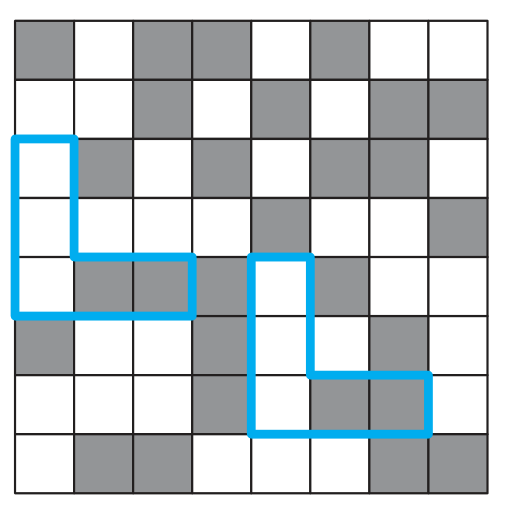
\includegraphics[scale=.5]{board.PNG}
\end{figure}







\vfill

\item (Hard) Let $n$ be a positive integer. Prove that for every square on a $2^n\times 2^n$ chess board, there is a tiling by $L$-triominoes (three squares that form a (possibly rotated) L-shape) of the remaining $4^n-1$ squares.

\vfill

\end{enumerate}

\end{document}